% \chapter{Appendix}
\chapter{Elasticsearch Related Information}
\section{Arxiv Parsed Research Index Example}

\begin{verbatim}
 {
    "identity": {
      "identity": "2104.00682",
      "url": "http://arxiv.org/abs/2104.00682v1",
      "title": "",
      "abstract": "",
      "categories": [
        "cs.CV",
        "cs.AI",
        "cs.LG"
      ],
      "published": "2021-04-01T17:59:48Z",
      "updated": "2021-04-01T17:59:48Z",
      "authors": [
        "Bo Xiong",
        "Haoqi Fan",
        "Kristen Grauman",
        "Christoph Feichtenhofer"
      ],
      "affiliation": [],
      "version": 1,
      "journal_reference": null,
      "created_on": "2021-04-02T04:20:33.981856"
    },
    "research_object": {
      "introduction": {
        "name": "Introduction",
        "subsections": [],
        "text": "",
        "matched": true
      },
      "related_works": {
        "name": "RelatedWorks",
        "subsections": [],
        "text": "",
        "matched": true
      },
      "methodology": {
        "name": "Methodology",
        "subsections": [],
        "text": "",
        "matched": false
      },
      "experiments": {
        "name": "Experiments",
        "subsections": [],
        "text": "",
        "matched": true
      },
      "results": {
        "name": "Results",
        "subsections": [],
        "text": "",
        "matched": false
      },
      "dataset": {
        "name": "Dataset",
        "subsections": [],
        "text": "",
        "matched": false
      },
      "conclusion": {
        "name": "Conclusion",
        "subsections": [],
        "text": "",
        "matched": true
      },
      "limitations": {
        "name": "Limitations",
        "subsections": [],
        "text": "",
        "matched": false
      },
      "unknown_sections": [
        {
          "name": "",
          "subsections": [
            {
              "name": "",
              "subsections": [],
              "text": ""
            }
          ],
          "text": ""
        }
      ]
    },
    "parsing_stats": {
      "active": true,
      "section_matches": [
        "Introduction",
        "RelatedWorks",
        "Experiments",
        "Conclusion"
      ],
      "num_un_matched": 2
    },
    "created_on": "2021-04-02T04:20:40.318679",
    "ontology": {
      "syntactic": [
      ],
      "semantic": [
      ],
      "union": [
      ],
      "enhanced": [
      ],
      "mined": true
    }
  }
\end{verbatim}
\pagebreak
\section{Content Parsing Code/Algorithm}
\label{appendix:content-parsing-code}
The \textit{ArxivLatexParser} is used to create the parsed content tree from which section based correlation is done. Below is the algorithm and source code in Python programming language.
\begin{lstlisting}
  
import os 
from subprocess import Popen, PIPE
from tex2py import tex2py 
from typing import List
import json


def get_tex_tree(tex_path):
    with open(tex_path,'r') as f:
        data = f.read()
    tex_root_node = tex2py(data)
    return tex_root_node

class Section():
    """Section 
    Section will contain subsections which are of type Section
    """
    def __init__(self,name=None):
        # Core Attributes
        self.name = self.__class__.__name__ if name is None else name
        self.subsections = [] # List[Sections]
        self.text = ''
    
    def to_markdown(self,tab_counter=0):
        SPACE= ' '
        HEADING='#'
        tab_counter+=1
        heading_val = HEADING*tab_counter if tab_counter <=3 else HEADING*3
        hierarchy = [heading_val+SPACE+self.name+"("+str(len(self.text))+")"]+[self._clean_text(self.text)] if len(self.text) > 0 else []
        for subsection in self.subsections:
            hierarchy.append(subsection.to_markdown(tab_counter=tab_counter))
        return '\n'.join(hierarchy)
    
    def to_quoted_tags(self):
        SPACE= ' '
        QUOTE_SECTION='<SECTION>'
        UNQUOTE_SECTION = '</SECTION>'
        QUOTE_CONTENT='\n<CONTENT>\n'
        UNQUOTE_CONTENT = '\n</CONTENT>\n'
        # tab_counter+=1
        # heading_val = HEADING*tab_counter if tab_counter <=3 else HEADING*3
        hierarchy = [
            QUOTE_SECTION+\
                self.name+UNQUOTE_SECTION]+[QUOTE_CONTENT+self._clean_text(self.text)+UNQUOTE_CONTENT] if len(self.text) > 0 else []
        for subsection in self.subsections:
            hierarchy.append(subsection.to_quoted_tags())
        return '\n'.join(hierarchy)

    @staticmethod
    def _clean_text(text):
        return text.replace('\\n','\n').replace('\t','').replace('\r','')
    
    def hierarchy_string(self,tab_counter=0):
        TAB = '\t'
        tab_counter+=1
        hierarchy = [TAB*tab_counter+self.name+"("+str(len(self.text.split(' ')))+")"]
        for subsection in self.subsections:
            hierarchy.append(subsection.hierarchy_string(tab_counter=tab_counter))
        return '\n'.join(hierarchy)
    
    def to_json(self):
        serialized_object = {
            'name' : self.name,
            'subsections': [],
            'text': self.text
        }
        for ss in self.subsections:
            serialized_object['subsections'].append(ss.to_json())
        return serialized_object

    @classmethod
    def from_json(cls,json_object):
        if 'name' not in json_object:
            raise SectionSerialisationException('"name" Attribute missing in object')
        generated_obj = cls(name=json_object['name'])
        generated_obj.text = json_object['text']
        for val in json_object['subsections']:
            generated_obj.subsections.append(cls.from_json(val))
        return generated_obj
    
    def save_to_file(self,file_path):
        with open(file_path,'w') as f:
            json.dump(self.to_json(),f)

    def _get_hierarchy(self):
        hierarchy = []
        for subsection in self.subsections:
            hierarchy.append(subsection._get_hierarchy())
        return {self.name:hierarchy}
        
    def __str__(self):
        return self.hierarchy_string()
    
    def flattened_sections(self):
        flattened_arr = []
        curr_sec = Section(name=self.name)
        curr_sec.text=self.text
        flattened_arr.append(curr_sec)
        for subsection in self.subsections:
            flattened_arr.extend(subsection.flattened_sections())
        return flattened_arr


class LatexParserException(Exception):
    headline = 'Latex Parsing failed'
    def __init__(self, msg='', lineno=None):
        self.message = msg
        self.line_no = lineno
        super(LatexParserException, self).__init__()

    def __str__(self):
        prefix = 'line %d: ' % self.line_no if self.line_no else ''
        return '%s%s' % (prefix, self.message)

class SectionSerialisationException(LatexParserException):
     def __init__(self,ms):
        msg = "Serialisation of Section Object Requires %s"%ms
        super(SectionSerialisationException, self).__init__(msg)

class LatexToTextException(LatexParserException):
    def __init__(self):
        msg = "Exception Raised From Text extraction at Detex"
        super(LatexToTextException, self).__init__(msg)


class DetexBinaryAbsent(LatexParserException):
    def __init__(self):
        msg = "Exception Raised Because Of No Detex Binary"
        super(DetexBinaryAbsent, self).__init__(msg)

class MaxSectionSizeException(LatexParserException):
    def __init__(self,avail,limit):
        msg = "Number of Sections %d are Larger than Maximum allowed (%d) for a Parsed Document"%(avail,limit)
        super(MaxSectionSizeException, self).__init__(msg)



class LatexToText():
    """LatexToText 
    This class will manage the conversion of the latex document into text. 
    It uses `detex` to extract the text from tex Files. 
    """
    detex_path = os.path.join(os.path.abspath(os.path.dirname(__file__)),'detex')

    def __init__(self,detex_path=None):
        # check binary existance. 
        if not self.binary_exists(self.detex_path):
            if detex_path is None:
                raise DetexBinaryAbsent()
            elif not self.binary_exists(detex_path):
                raise DetexBinaryAbsent()
            else:
                self.detex_path = detex_path
        
    @staticmethod
    def binary_exists(detex_path):
        try:
            os.stat(detex_path)
        except:
            return False
        return True
    
    def __call__(self,latex_document_path):
        try:
            process = Popen([self.detex_path, latex_document_path], stdout=PIPE)
            (output, err) = process.communicate()
            exit_code = process.wait()
            return output
        except Exception as e:
            print(e)
            raise LatexToTextException()

def split_match(split_value:str,splitting_string:str,split_upto=0.5,split_bins=10):
    """split_match 
    Splits a Keep Splitting a `splitting_string` based on the value of `split_value`.
    It does so by removing `split_upto`% of the string until there is a match. or return no match. 
    
    `split_upto` specifies the size after which it will stop splitting. 

    :param split_value: [String]
    :param splitting_string: [description]
    :param split_upto: [float], defaults to 0.5 
    :param split_bins: [int] the number bins inside which each `split_value` will fall under. 
                                eg. 
                                    split_value = "Deep Learning Techniques for ASD Diagnosis and Rehabilitation'"
                                    split_bins=3,
                                    split_upto=0.5
                                    then the text will be checked for matches against : 
                                        - ['Deep Learning Techniques for','Deep Learning Techniques for ASD','Deep Learning Techniques for ASD Diagnosis','Deep Learning Techniques for ASD Diagnosis and' ....]
                                        - The purpose of doing this is to ensure a partial match of a string can help extract the split text 
    :returns splitted_text : List[String] : [s1,s2] or []
    """
    split_value = split_value.split(' ') # This make it remove words instead of the characters. 
    sb = [i for i in range(split_bins)]
    split_mul = (1-split_upto)/split_bins
    # Spread the `split_bins` according to the how much the split needs to happen. 
    split_range = [1-float((i)*split_mul) for i in sb]
    # index at which the new `split_value` will be determined. Order is descending to ensure largest match. 
    slice_indices = [int(len(split_value)*split_val) for split_val in split_range] 
    # creates the split strings.     
    split_values_to_checks = [' '.join(split_value[:index]) for index in slice_indices] 
    
    for split_val in split_values_to_checks:
        if split_val == '': # In case of empty seperator leaave it. 
            continue
        current_text_split = splitting_string.split(split_val)
        if len(current_text_split) > 1:
            return current_text_split
    
    return []

class LatexInformationParser(object):
    """LatexInformationParser 

    This is the parent class responsible for extraction of Processed information from 
    Latex Based Documents. Process follows the below steps:

    ## `section_extraction`
    Use the `section_extraction` method to extract the document information
    sections from the single/document Latex setup. This returns a Sequential Tree like structure with sub sequences. 
    This will use `tex2py` like functions to extract the document structure from the tex documents. 
    
    ## `text_extraction`:
    Will extract text from the Latex File. uses `opendetex` to extract the text from latex. 

    ## `collate_sections` : 
    This will collate the information text and sections extracted based on the strategy of the extraction. 

    """
    max_section_limit = 30 # Maximum number of sections to allow for extraction
    def __init__(self,max_section_limit=20,detex_path=None):
        self.max_section_limit = max_section_limit
        self.text_extractor = LatexToText(detex_path=detex_path)

    
    def section_extraction(self,tex_file_path) -> List[Section]:
        raise NotImplementedError()
    
    @staticmethod
    def get_subsection_names(tex_node):
        subsections = []
        try:
            subsections = list(tex_node.subsections)
            subsections = [i.string for i in subsections]
        except:
            pass
        return subsections            


    def text_extraction(self):
        raise NotImplementedError()

    def collate_sections(self):
        raise NotImplementedError()

    def from_arxiv_paper(self,tex_files):
        raise NotImplementedError()


class SingleDocumentLatexParser(LatexInformationParser):
    def __init__(self, max_section_limit=20,detex_path=None):
        super().__init__(max_section_limit=max_section_limit,detex_path=detex_path)
    
    def section_extraction(self,tex_file_path) -> List[Section]:
        tex_node = get_tex_tree(tex_file_path)
        if len(tex_node.branches) > self.max_section_limit:
            raise MaxSectionSizeException(len(tex_node.branches),self.max_section_limit)
        
        sequential_sections = []
        for node in tex_node:
            curr_section = Section(str(node))
            subsections = self.get_subsection_names(node)
            curr_section.subsections = [Section(ss) for ss in subsections]
            sequential_sections.append(curr_section)

        return sequential_sections
    
    def text_extraction(self,latex_path):
        return self.text_extractor(latex_path)

            
    @staticmethod
    def split_and_find_section(curr_text,curr_sec_name,prev_section,split_upto=0.2,split_bins=10):
        """split_and_find_section 
        Helps Recurrsively/iteratively split a Latex document for the Section list found from 
        `section_extraction`. Splits a text string based on `curr_sec_name` and then allocates the 
        split[0] to the `prev_section` object. 
        
        :type curr_text: [String]
        :type curr_sec_name: [String]
        :type prev_section: [Section]
        :type split_upto : refer `split_match`
        :type split_bins : refer `split_match`
        :returns curr_text,Find_status : After removal of redundant section post splitting. 
                                         status points to weather it could set text of the 
                                         `prev_section` object
        """
        current_text_split = split_match(curr_sec_name,curr_text,split_upto=split_upto,split_bins=split_bins)
        # print("Found Splits,",curr_sec_name,len(current_text_split))
        if len(current_text_split) == 0: 
            # This means no splits were found 
            return curr_text,False

        portion_before_section = current_text_split[0] 

        if prev_section is not None:
            prev_section.text = portion_before_section
            # print(ss.name,"added To Section ",prev_section.name,len(prev_section.text))
        portion_after_section = current_text_split[1:]
        curr_text = ''.join(portion_after_section)
        return curr_text,True

    
    def collate_sections(self,paper_text,section_list:List[Section],split_upto=0.2,split_bins=10):
        """collate_sections 
        Gets Latex compiled text string and 
        then uses the found section based hierarchy from Latex
        to fill Text content of the `Section` objects which were discovered in 
        `section_extraction`

        :param paper_text: text in string of from text_extraction]
        :type section_list: List[Section]
        :return: List[Section] : filled with text attributed
        """
        current_text_split = []
        prev_section = None
        curr_text = str(paper_text)
        unfound_sections = []
        some_section_not_found = False
        for index,s in enumerate(section_list):
            curr_text,section_status = self.split_and_find_section(curr_text,s.name,prev_section,split_upto=split_upto,split_bins=split_bins)
            if not section_status: # If couldn't match section add it here. 
                some_section_not_found = True
            # print('\n\t'+s.name)                
            prev_section = s 
            for ss in s.subsections:
                curr_text,section_status = self.split_and_find_section(curr_text,ss.name,prev_section,split_upto=split_upto,split_bins=split_bins)
                if not section_status:
                    some_section_not_found = True
                    # print("Cannot Match For :",ss.name)
                prev_section = ss
                # print('\n\t\t'+ss.name)
            if index == len(section_list)-1:
                s.text = curr_text
        return section_list,some_section_not_found
    
    def from_arxiv_paper(self,tex_files:List[str],lowest_section_match_percent=0.2,number_to_tries=10):
        """from_arxiv_paper 
        Extract Parsable section array from Arxiv Latex Paper which only have one paper will all the sections in it. 
        :param lowest_section_match_percent [float]: % of the section heading that mimimum matches to create the split in text for parsing. 
        :param paper: [ArxivPaper]
        :param number_to_tries: [float], number of different matches to make with mimimum match strings
        :return: Tuple (
            found_sections:List[Section],
            some_section_not_found:bool,
            latex_files_status_dict:dict
        ) 
        """
        largest_file = None
        max_size = 0
        file_results = {}
        for file_path in tex_files:
            if os.path.getsize(file_path) > max_size:
                largest_file = file_path
        latex_path = largest_file
        sections = self.section_extraction(latex_path)
        tex_in_text = self.text_extraction(latex_path)
        sections,some_section_not_found = self.collate_sections(tex_in_text,sections,split_upto=lowest_section_match_percent,split_bins=number_to_tries)
        file_results[latex_path] = some_section_not_found
        return sections,some_section_not_found,file_results

class MultiDocumentLatexParser(SingleDocumentLatexParser):
    def __init__(self, max_section_limit=20, detex_path=None):
        super().__init__(max_section_limit=max_section_limit, detex_path=detex_path)
    

    def from_arxiv_paper(self,tex_files:List[str],lowest_section_match_percent=0.2,number_to_tries=10):
        """from_arxiv_paper 
        Extract Parsable section array from Arxiv Latex Paper which only have one paper will all the sections in it. 
        :param tex_files: [path to files]
        :param lowest_section_match_percent [float]: % of the section heading that mimimum matches to create the split in text for parsing. 
        :param number_to_tries: [float], number of different matches to make with mimimum match strings
        :return: Tuple (
            found_sections:List[Section],
            some_section_not_found:bool,
            latex_files_status_dict:dict
        ) 
        """
        collected_sections = []
        snf = False
        file_results = {}
        for latex_path in tex_files:
            try:
                sections = self.section_extraction(latex_path)
                tex_in_text = self.text_extraction(latex_path)
                sections,some_section_not_found = self.collate_sections(tex_in_text,sections,split_upto=lowest_section_match_percent,split_bins=number_to_tries)
                file_results[latex_path] = True
                if some_section_not_found:
                    snf = some_section_not_found
                collected_sections+=sections
            except:
                file_results[latex_path] = False
        return collected_sections,snf,file_results

class ArxivLatexParser():
    """
    Parses Arxiv Latex Documents with `LatexInformationParser` according 
        - Based on Number of latex Pages (Chooses `SingleDocumentLatexParser` | `MultiDocumentLatexParser`)
            - Parsing is Ment to create Tree Like `Section` Datastructures.  
    
    :return: tuple(
        collected_sections:List[Section],
        some_sections_failed:bool,
        file_results:dict
    )
    """
    parsing_result_name = 'Symantic Parsing Result'

    def __init__(self,max_section_limit=20, detex_path=None):
        self.single_doc_parser = SingleDocumentLatexParser(max_section_limit=max_section_limit, detex_path=detex_path)
        self.multi_doc_parser = MultiDocumentLatexParser(max_section_limit=max_section_limit, detex_path=detex_path)
    
    def __call__(self,tex_files:List[str],lowest_section_match_percent=0.2,number_to_tries=10):
        selected_parser = None
        if len(tex_files) == 0 : 
           return None
        
        # Selected Parser for Latex based On Size.            
        if len(tex_files) >=4:
            selected_parser = self.multi_doc_parser
        elif len(tex_files) >=1:
            selected_parser = self.single_doc_parser
        
        # Run the parser and see the results. 
        try:
            collected_sections,some_sections_failed,file_results = selected_parser.from_arxiv_paper(tex_files,lowest_section_match_percent=lowest_section_match_percent,number_to_tries=number_to_tries)
            return collected_sections,some_sections_failed,file_results
        except Exception as e:
            return None
        
      

\end{lstlisting}
\pagebreak
\section{Heuristic Mapping Values For Serialisation of Research Object}
\label{appendix:mapping-heuristic}
\begin{lstlisting}
  INTRODUCTION_SEARCH_CONSTS = [
    "introduction",
    "preliminaries",
    
]
RELATED_WORKS_SEARCH_CONSTS = [
    "problem statement",
    "background",
    "related work",
    "problem definition",
    "literature review",

]
METHODOLOGY_SEARCH_CONST = [
    "methodology",
    "method",
    "problem formulation",
    "approach",
    "proposed method"
    "implementation",
    "our approach",
    "proposed algorithm",
    "system design",
    "architecture",

]
DATA_SEARCH_CONST = [
    "dataset",
    "data"
]

EXPERIMENTS_SEARCH_CONSTS = [
    "evaluation",
    "experiment",
]
RESULTS_SEARCH_CONSTS = [
    'result',
    "analysis"
]

CONCLUSION_SEARCH_CONSTS = [
    "discussion",
    "conclusion",
    "future work",
    "concluding remarks"
]

LIMITATIONS_SEARCH_CONSTS = [
    "limitations",
    "ablation study",

]

STRICT_CHECK_CONSTS = [
    "data", # These key words need strict "==" checking to ensure the match name
    "method",
    "approach"
]
\end{lstlisting}

\chapter{Table Of Comparison Classification}
\label{appendix:toc}
\section{Hyper Parameters For ML Training}
\begin{table}[h]
  \label{table\arabic{tablecounter}}
  \centering
  \begin{tabular}{|p{1.25cm}|p{1.25cm}|p{1.75cm}|p{1.5cm}|p{1.5cm}|p{1.5cm}|p{1cm}|p{1cm}|}
  \hline
      Model Name & \#  Layers &  Embedding Size & Batchsize & Learning Rate & \#  Parameters & Size In MB & \# Epoch\\ \hline
      CCT (31M) & 6 Layers Per Cross Channel, 6 Layers Per Vanilla Encoder & 256 & 8 & 2e-05 & 31M & 140 & 20\\ \hline
      E-MCT (25M) & 8 Vanilla Encoder & 256 & 8 & 2e-05 & 25M & 100 & 20\\ \hline
      Caption Only Encoder Transformer (14.5M) & 8 Vanilla Encoder & 256 & 8 & 2e-05 & 14.5M & 58 & 20\\ \hline
      SciBert Finetuned & 12 Vanilla Encoder Layers & 768 & 8 & 2e-05 & 109 M & 440 & 6 \\ \hline
  \end{tabular}
  \caption{\label{tablecounter} Hyper Parameters For Training Table Classification Models. All Learning rates are scheduled using a cosine learning rate scheduler with a warm up of 20 epochs. }
\end{table}
\refstepcounter{tablecounter}


\section{Table Type Examples}
\label{appendix:toc:type-exp}
% Figure \ref{figure}
The examples of the types of tables labeled during the labeling processs are given in Figure \ref{figure30}, \ref{figure31}, \ref{figure32}, \ref{figure33}, \ref{figure34}, \ref{figure35}. 
\begin{figure}[h!]
    \centering
    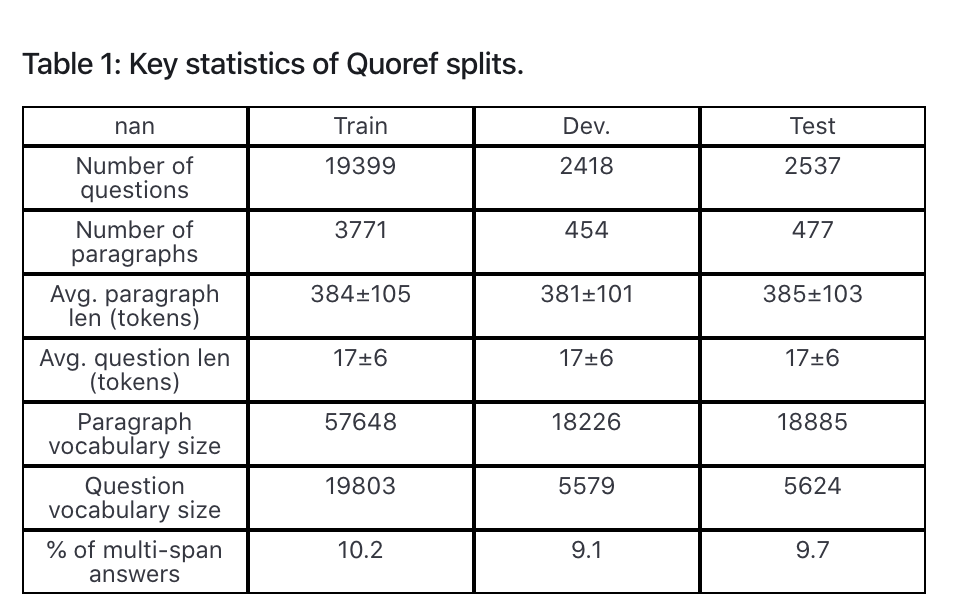
\includegraphics[width=\maxwidth{\textwidth}]{src/images/type-exp-ds-stat.png}
    \legend{\emph{Source}: From \cite{dasigi2019quoref}}
    \caption{Table Type : Dataset Description. }
    \label{figure\arabic{figurecounter}}
\end{figure}
\refstepcounter{figurecounter}

\begin{figure}[h!]
    \centering
    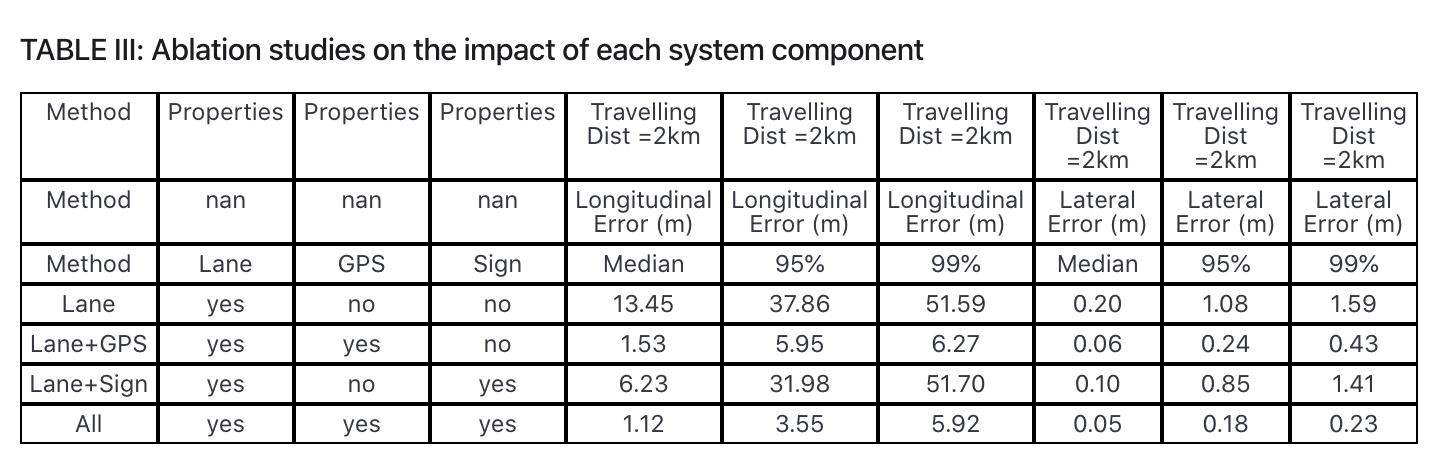
\includegraphics[width=\maxwidth{\textwidth}]{src/images/type-exp-ablation.png}
    \legend{\emph{Source}: From \cite{ma2019exploiting}}
    \caption{Table Type : Ablation Study. }
    \label{figure\arabic{figurecounter}}
\end{figure}
\refstepcounter{figurecounter}

\begin{figure}[h!]
    \centering
    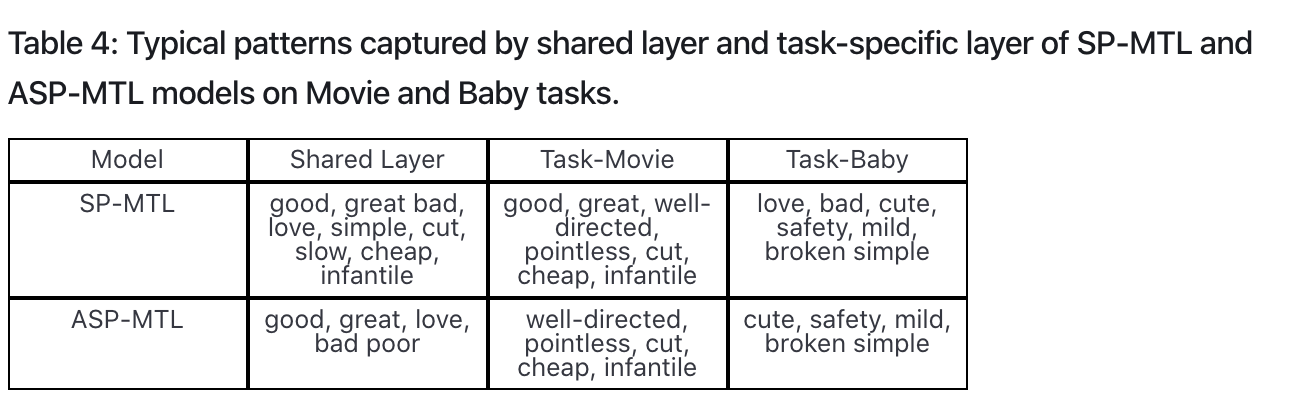
\includegraphics[width=\maxwidth{\textwidth}]{src/images/type-exp-method.png}
    \legend{\emph{Source}: From \cite{liu2017adversarial}}
    \caption{Table Type : Method Examples.}
    \label{figure\arabic{figurecounter}}
\end{figure}
\refstepcounter{figurecounter}

\begin{figure}[h!]
    \centering
    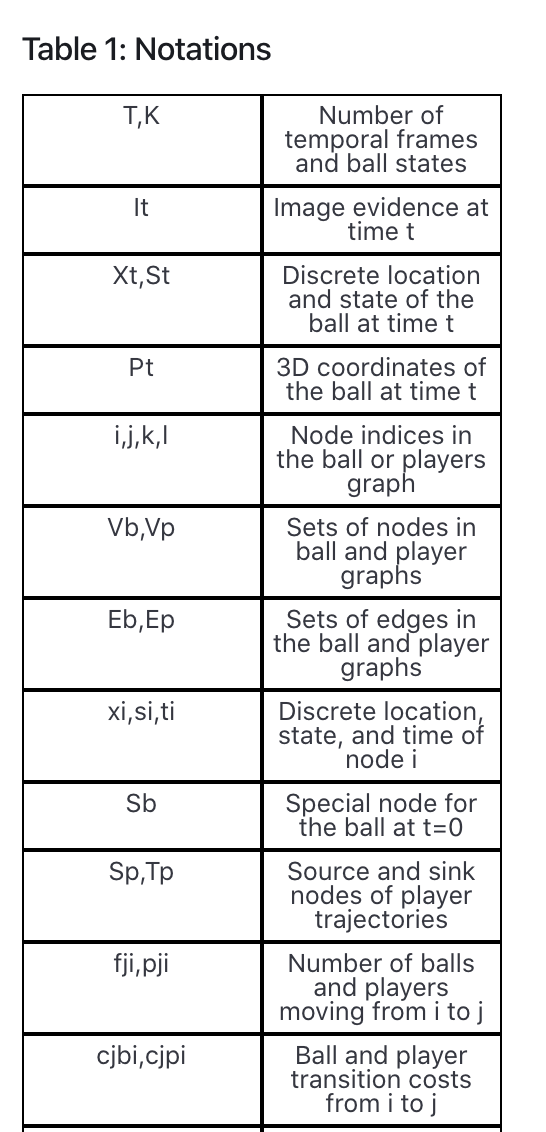
\includegraphics[width=\maxwidth{0.5\textwidth}]{src/images/type-exp-symbolic.png}
    \legend{\emph{Source}: From \cite{maksai2016players}}
    \caption{Table Type : Symbolic Parameter Description. }
    \label{figure\arabic{figurecounter}}
\end{figure}
\refstepcounter{figurecounter}

\begin{figure}[h!]
    \centering
    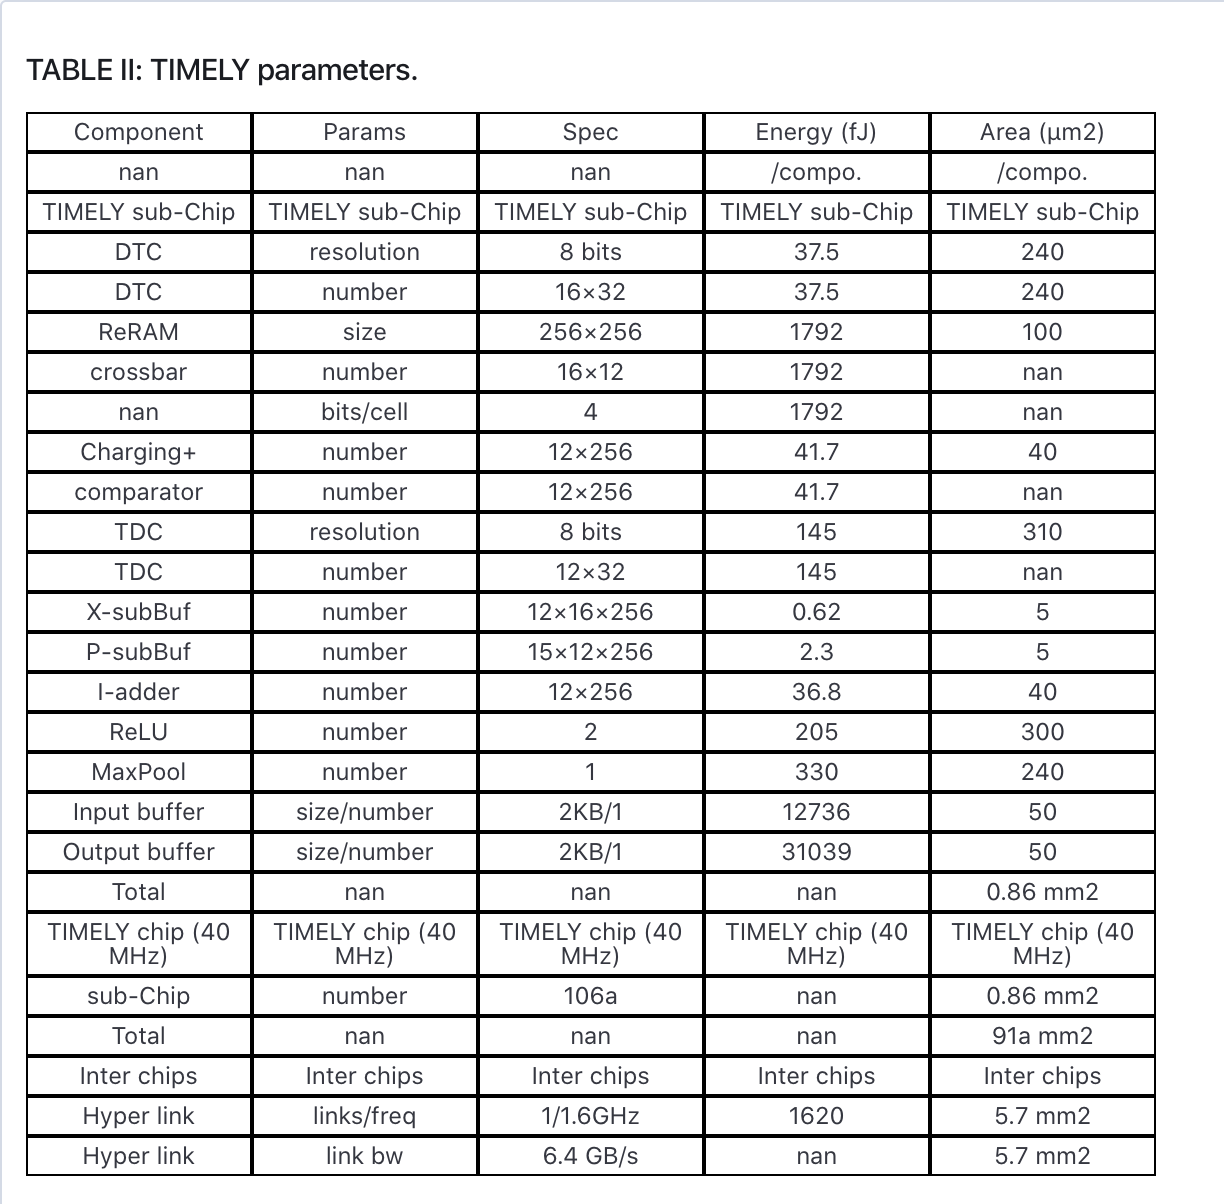
\includegraphics[width=\maxwidth{\textwidth}]{src/images/type-exp-hparam.png}
    \legend{\emph{Source}: From \cite{maksai2016players}}
    \caption{Table Type : HyperParameter Description.}
    \label{figure\arabic{figurecounter}}
\end{figure}
\refstepcounter{figurecounter}


\begin{figure}[h!]
    \centering
    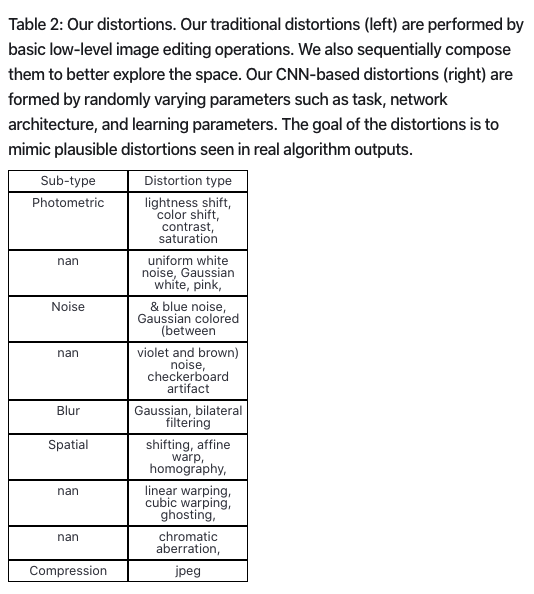
\includegraphics[width=\maxwidth{\textwidth}]{src/images/type-exp-param.png}
    \legend{\emph{Source}: From \cite{zhang2018unreasonable}}
    \caption{Table Type : Parameter Description.}
    \label{figure\arabic{figurecounter}}
\end{figure}
\refstepcounter{figurecounter}

